\section{Casi d'uso}
	Per i casi d'uso verranno utilizzate le seguenti sigle:
	\begin{itemize}
		\item \textbf{[UNA]}: Utente non autenticato;
		\item \textbf{[UA]}: Utente autenticato;
		\item \textbf{[ME]}: Moderatore ente;
		\item \textbf{[AM]}: Amministratore.
	\end{itemize}

		
		% =================
		% UC 1

			\subsection{UC1 - Web App - Autenticazione}
		
	\begin{figure}[H]
		\centering
		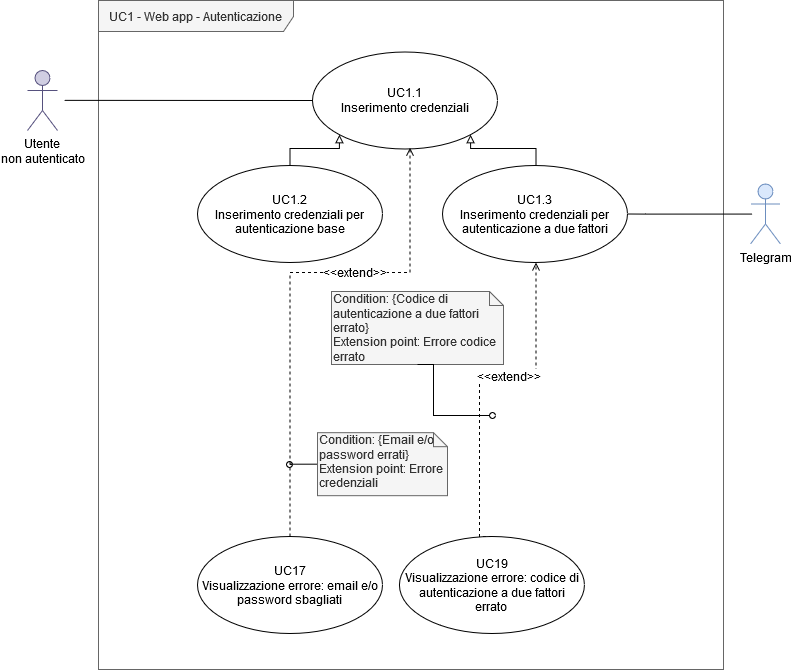
\includegraphics[scale=0.60]{res/images/uc1}
		\caption{Diagramma che riassume il processo di autenticazione nella web app.}
	\end{figure}
		
	\begin{itemize}
		\item \textbf{Attori Primari}: Utente non autenticato.
		\item \textbf{Attori Secondari}: \glock{Telegram}.
		\item \textbf{Descrizione}: L'utente vuole autenticarsi nella web app, per poter accedere alle funzionalità del sito.
		\item \textbf{Precondizione}: L'utente non è autenticato nella web app.
		\item \textbf{Postcondizione}: L'utente effettua l'autenticazione nella web app.
		\item \textbf{Scenario Principale}:
		\begin{enumerate}
			\item L'utente inserisce le proprie credenziali (UC 1.1);
			\item Viene eseguito il controllo delle credenziali inserite (UC 1.4).
		\end{enumerate}
	\end{itemize}
	

		\subsubsection{UC 1.1 - Inserimento credenziali}

		\begin{itemize}
			\item \textbf{Attori Primari}: Utente non autenticato.
			\item \textbf{Descrizione}: L'utente vuole autenticarsi nella web app e deve inserire alcuni campi obbligatori per procedere.
			\item \textbf{Precondizione}: L'utente non è autenticato nella web app.
			\item \textbf{Postcondizione}: L'utente ha inserito le credenziali richieste.
			\item \textbf{Scenario Principale}:
			\begin{enumerate}
				\item L'utente inserisce le credenziali per l'autenticazione base (UC 1.2);
				\item L'utente inserisce le credenziali per l'autenticazione a due fattori (UC 1.3);
			\end{enumerate}
			\item \textbf{Inclusioni}:
				\begin{itemize}
					\item Controllo credenziali (UC 1.4).
				\end{itemize}
			\item \textbf{Estensioni}:
				\begin{itemize}
					\item Visualizzazione errore: email e/o una password errati (UC 17).
				\end{itemize}
		\end{itemize}

		\subsubsection{UC 1.2 - Inserimento credenziali per autenticazione base}

		\begin{figure}[H]
			\centering
			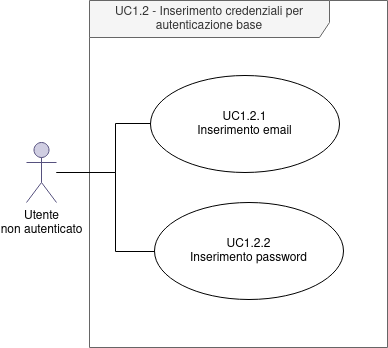
\includegraphics[scale=0.675]{res/images/uc1.2}
			\caption{Diagramma che descrive l'inserimento delle credenziali per l'autenticazione base.}
		\end{figure}

		\begin{itemize}
			\item \textbf{Attori Primari}: Utente non autenticato.
			\item \textbf{Descrizione}: L'utente vuole autenticarsi nella web app ed inserisce i campi obbligatori per l'autenticazione base.
			\item \textbf{Precondizione}: L'utente non è autenticato nella web app.
			\item \textbf{Postcondizione}: L'utente ha inserito le credenziali richieste.
			\item \textbf{Scenario Principale}:
			\begin{enumerate}
				\item L'utente inserisce la email (UC 1.2.1);
				\item L'utente inserisce la password (UC 1.2.2).
			\end{enumerate}	
		\end{itemize}

			\paragraph{UC 1.2.1 - Inserimento email}
			\begin{itemize}
				\item \textbf{Attori Primari}: Utente non autenticato.
				\item \textbf{Descrizione}: L'utente vuole autenticarsi nella web app e inserisce uno dei campi obbligatori per l'autenticazione base.
				\item \textbf{Precondizione}: L'utente non è autenticato nella web app.
				\item \textbf{Postcondizione}: L'utente ha inserito la credenziale richiesta.
				\item \textbf{Scenario Principale}:
				\begin{enumerate}
					\item L'utente compila il campo email.
				\end{enumerate}	
			\end{itemize}

			\paragraph{UC 1.2.2 - Inserimento password}
			\begin{itemize}
				\item \textbf{Attori Primari}: Utente non autenticato.
				\item \textbf{Descrizione}: L'utente vuole autenticarsi nella web app e inserisce uno dei campi obbligatori per l'autenticazione base.
				\item \textbf{Precondizione}: L'utente non è autenticato nella web app.
				\item \textbf{Postcondizione}: L'utente ha inserito la credenziale richiesta.
				\item \textbf{Scenario Principale}:
				\begin{enumerate}
					\item L'utente compila il campo password.
				\end{enumerate}	
			\end{itemize}

		\subsubsection{UC 1.3 - Inserimento credenziali per autenticazione a due fattori}

		\begin{figure}[H]
			\centering
			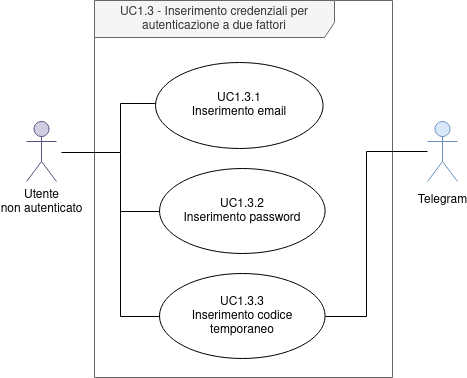
\includegraphics[scale=0.675]{res/images/uc1.3}
			\caption{Diagramma che descrive l'inserimento delle credenziali per l'autenticazione a due fattori.}
		\end{figure}

		\begin{itemize}
			\item \textbf{Attori Primari}: Utente non autenticato.
			\item \textbf{Attori Secondari}: \glock{Telegram}.
			\item \textbf{Descrizione}: L'utente vuole autenticarsi nella web app ed inserisce i campi obbligatori per l'autenticazione a due fattori.
			\item \textbf{Precondizione}: L'utente non è autenticato nella web app.
			\item \textbf{Postcondizione}: L'utente ha inserito le credenziali richieste.
			\item \textbf{Scenario Principale}:
				\begin{enumerate}
					\item L'utente inserisce la email (UC 1.3.1);
					\item L'utente inserisce la password (UC 1.3.2);
					\item L'utente inserisce un codice temporaneo ricevuto tramite \glock{Telegram} (UC 1.3.3).
				\end{enumerate}
			\item \textbf{Estensioni}:
				\begin{itemize}
					\item Visualizzazione errore: codice di autenticazione a due fattori errato (UC 19).
				\end{itemize}	
		\end{itemize}

			\paragraph{UC 1.3.1 - Inserimento email}
			\begin{itemize}
				\item \textbf{Attori Primari}: Utente non autenticato.
				\item \textbf{Descrizione}: L'utente vuole autenticarsi nella web app e inserisce uno dei campi obbligatori per l'autenticazione a due fattori.
				\item \textbf{Precondizione}: L'utente non è autenticato nella web app.
				\item \textbf{Postcondizione}: L'utente ha inserito la credenziale richiesta.
				\item \textbf{Scenario Principale}:
				\begin{enumerate}
					\item L'utente compila il campo email.
				\end{enumerate}	
			\end{itemize}

			\paragraph{UC 1.3.2 - Inserimento password}
			\begin{itemize}
				\item \textbf{Attori Primari}: Utente non autenticato.
				\item \textbf{Descrizione}: L'utente vuole autenticarsi nella web app e inserisce uno dei campi obbligatori per l'autenticazione a due fattori.
				\item \textbf{Precondizione}: L'utente non è autenticato nella web app.
				\item \textbf{Postcondizione}: L'utente ha inserito la credenziale richiesta.
				\item \textbf{Scenario Principale}:
				\begin{enumerate}
					\item L'utente compila il campo password.
				\end{enumerate}	
			\end{itemize}

			\paragraph{UC 1.3.3 - Inserimento codice temporaneo}
			\begin{itemize}
				\item \textbf{Attori Primari}: Utente non autenticato.
				\item \textbf{Attori Secondari}: \glock{Telegram}.
				\item \textbf{Descrizione}: L'utente vuole autenticarsi nella web app e inserisce uno dei campi obbligatori per l'autenticazione a due fattori.
				\item \textbf{Precondizione}: L'utente non è autenticato nella web app.
				\item \textbf{Postcondizione}: L'utente ha inserito la credenziale richiesta.
				\item \textbf{Scenario Principale}:
				\begin{enumerate}
					\item L'utente riceve una notifica tramite \glock{Telegram} con un codice temporaneo;
					\item L'utente compila il campo codice temporaneo.
				\end{enumerate}	
			\end{itemize}


		
		% =================
		% UC 2

		\subsubsection{UC 2 - Visualizzazione dashboard e menù}
		
		\begin{itemize}
			\item \textbf{Attori Primari}: utente autenticato, moderatore ente, amministratore;
			\item \textbf{Descrizione}: L'utente ha eseguito l'autenticazione e visualizza la dashboard con le funzionalità di cui dispone i permessi.
			\item \textbf{Precondizione}: L'utente ha eseguito  con successo l'autenticazione.
			\item \textbf{Postcondizione}: L'utente visualizza la dashboard con il contenuto basato sull'attore autenticato.
			\item \textbf{Scenario Principale}:
			\begin{enumerate}
				\item L'utente ha eseguito l'autenticazione;
				\item L'utente visualizza la dashboard e il menù.
			\end{enumerate}	
		\end{itemize}

		% =================
		% UC 3

		\subsubsection{UC 3 - Logout}
		\begin{itemize}
			\item \textbf{Attori Primari}: utente autenticato, moderatore ente, amministratore;
			\item \textbf{Descrizione}: L'utente effettua l'uscita dalla web-application diventando l'attore \textit{Utente non autenticato}.
			\item \textbf{Precondizione}: L'utente seleziona la voce \textit{logout}.
			\item \textbf{Postcondizione}: L'utente visualizza la schermata di login.
			\item \textbf{Scenario Principale}:
			\begin{enumerate}
				\item l'utente seleziona la voce \textit{logout};
				\item L'utente effettua il logout;
				\item L'utente visualizza la schermata di login.
			\end{enumerate}	
		\end{itemize}

		% =================
		% UC 4 - DA FARE

			\subsection{UC 4 - Impostazioni Account}
		
		\begin{figure}[H]
			\centering
			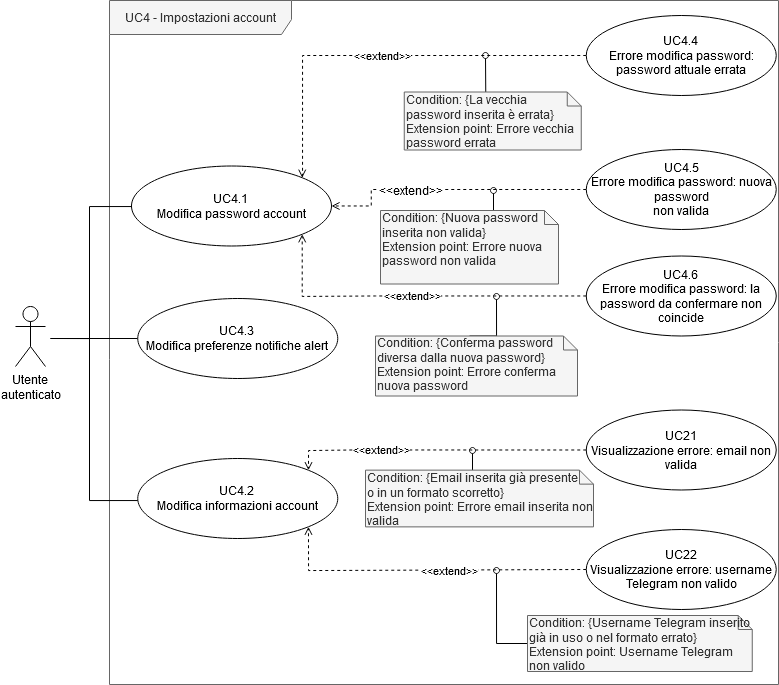
\includegraphics[scale=0.60]{res/images/uc4}
			\caption{Diagramma che riassume le interazioni con le impostazioni del proprio account.}
		\end{figure}
		
		\begin{itemize}
			\item \textbf{Attori Primari}: Utente autenticato.
			\item \textbf{Descrizione}: L'utente ha la possibilità di gestire le proprie impostazioni account, tra cui la modifica della password, le preferenze di notifica e le informazioni a lui associate.
			\item \textbf{Precondizione}: L'utente risulta autenticato all'interno della web app.
			\item \textbf{Postcondizione}: L'utente ha aggiornato le proprie impostazioni.
			\item \textbf{Scenario Principale}:
			\begin{enumerate}
				\item{L'utente naviga all'interno delle impostazioni del proprio account}
				\item{L'utente modifica le proprie impostazioni}
				\item{L'utente ha aggiornato le proprie impostazioni}
			\end{enumerate}	
		\end{itemize}
			

			\subsubsection{UC 4.1 - Modifica password account}
			\begin{itemize}
				\item \textbf{Attori Primari}: Utente autenticato.
				\item \textbf{Descrizione}: L'utente può cambiare la password associata al proprio account.
				\item \textbf{Precondizione}: L'utente naviga all'interno delle sue impostazioni.
				\item \textbf{Postcondizione}: L'utente ha cambiato la propria password.
				\item \textbf{Scenario Principale}:
				\begin{enumerate}
					\item L'utente deve inserire dei campi obbligatori per proseguire;
					\item L'utente inserisce il campo per la password attuale (4.1.1);
					\item L'utente inserisce il campo per la nuova password (4.1.2);
					\item L'utente inserisce il campo per la conferma della nuova password (4.1.3);
					\item L'utente ha cambiato la propria password.
				\end{enumerate}	
				\item \textbf{Estensioni}:
					\begin{itemize}
						\item Errore modifica password: password attuale errata (UC 4.4)
						\item Errore modifica password: nuova password non valida (UC 4.5)
						\item Errore modifica password: la password da confermare non coincide co la nuova password (UC 4.6)
					\end{itemize}
			\end{itemize}

				\paragraph{UC 4.1.1 - Inserimento password attuale}
				\begin{itemize}
					\item \textbf{Attori Primari}: Utente autenticato.
					\item \textbf{Descrizione}: Per proseguire nella modifica password, l'utente deve inserire la sua password attuale associata all'account. Il campo è obbligatorio.
					\item \textbf{Precondizione}: L'utente è all'interno delle sue impostazioni account.
					\item \textbf{Postcondizione}: L'utente ha compilato il campo richiesto.
					\item \textbf{Scenario Principale}:
					\begin{enumerate}
						\item L'utente compila il campo per la password attuale.
					\end{enumerate}
				\end{itemize}

				\paragraph{UC 4.1.2 - Inserimento nuova password}
				\begin{itemize}
					\item \textbf{Attori Primari}: Utente autenticato.
					\item \textbf{Descrizione}: Per proseguire nella modifica password, l'utente deve scegliere e inserire una nuova password. Il campo è obbligatorio.
					\item \textbf{Precondizione}: L'utente è all'interno delle sue impostazioni account.
					\item \textbf{Postcondizione}: L'utente ha compilato il campo richiesto.
					\item \textbf{Scenario Principale}:
					\begin{enumerate}
						\item L'utente compila il campo per la nuova password.
					\end{enumerate}
				\end{itemize}

				\paragraph{UC 4.1.3 - Inserimento conferma nuova password}
				\begin{itemize}
					\item \textbf{Attori Primari}: Utente autenticato.
					\item \textbf{Descrizione}: Per proseguire nella modifica password, l'utente deve ripetere la nuova password scelta. Il campo è obbligatorio.
					\item \textbf{Precondizione}: L'utente è all'interno delle sue impostazioni account.
					\item \textbf{Postcondizione}: L'utente ha compilato il campo richiesto.
					\item \textbf{Scenario Principale}:
					\begin{enumerate}
						\item L'utente compila il campo per la conferma della nuova password.
					\end{enumerate}
				\end{itemize}

			\subsubsection{UC 4.2 - Modifica informazioni account}
			\begin{itemize}
				\item \textbf{Attori Primari}: Utente autenticato.
				\item \textbf{Descrizione}: L'utente può modificare le proprie informazioni associate all'account.
				\item \textbf{Precondizione}: L'utente naviga all'interno delle sue impostazioni.
				\item \textbf{Postcondizione}: L'utente ha cambiato le proprie informazioni account.
				\item \textbf{Scenario Principale}:
				\begin{enumerate}
					\item L'utente deve inserire dei campi per proseguire;
					\item L'utente modifica il campo relativo alla propria email (4.2.1);
					\item L'utente modifica il campo relativo allo username di \glock{Telegram} (4.2.2);
					\item L'utente seleziona la preferenza per l'abilitazione dell'autenticazione a due fattori (4.2.3);
					\item L'utente ha cambiato le proprie informazioni associate al suo account.
				\end{enumerate}	
				\item \textbf{Estensioni}:
					\begin{itemize}
						\item L'utente inserisce un'email non valida (UC 21);
						\item L'utente inserisce uno username \glock{Telegram} non valido (UC 22).
					\end{itemize}
			\end{itemize}

				\paragraph{UC 4.2.1 - Modifica della propria email}
				\begin{itemize}
					\item \textbf{Attori Primari}: Utente autenticato.
					\item \textbf{Descrizione}: Per proseguire nella modifica delle informazioni, l'utente deve modificare il campo della propria email. Il campo è obbligatorio.
					\item \textbf{Precondizione}: L'utente è all'interno delle sue impostazioni account.
					\item \textbf{Postcondizione}: L'utente ha compilato il campo richiesto.
					\item \textbf{Scenario Principale}:
					\begin{enumerate}
						\item L'utente compila il campo per la email.
					\end{enumerate}
				\end{itemize}

				\paragraph{UC 4.2.2 - Modifica dello username Telegram}
				\begin{itemize}
					\item \textbf{Attori Primari}: Utente autenticato.
					\item \textbf{Descrizione}: Per proseguire nella modifica delle informazioni, l'utente deve modificare il proprio username \glock{Telegram}. Il campo è obbligatorio.
					\item \textbf{Precondizione}: L'utente è all'interno delle sue impostazioni account.
					\item \textbf{Postcondizione}: L'utente ha compilato il campo richiesto.
					\item \textbf{Scenario Principale}:
					\begin{enumerate}
						\item L'utente compila il campo dello username \glock{Telegram}.
					\end{enumerate}
				\end{itemize}

				\paragraph{UC 4.2.3 - Modifica delle preferenze per l'autenticazione a due fattori}
				\begin{itemize}
					\item \textbf{Attori Primari}: Utente autenticato.
					\item \textbf{Descrizione}: Per proseguire nella modifica delle informazioni, l'utente deve selezionare le preferenze per l'abilitazione o meno dell'autenticazione a due fattori con \glock{Telegram}. Le preferenze disponibili sono:
					\begin{itemize}
						\item Abilitata;
						\item Disabilitata.
					\end{itemize}
					\item \textbf{Precondizione}: L'utente è all'interno delle sue impostazioni account.
					\item \textbf{Postcondizione}: L'utente ha compilato il campo richiesto.
					\item \textbf{Scenario Principale}:
					\begin{enumerate}
						\item L'utente seleziona la preferenza per l'autenticazione a due fattori.
					\end{enumerate}
				\end{itemize}


			\subsubsection{UC 4.3 - Modifica preferenze notifiche alert}
			\begin{itemize}
				\item \textbf{Attori Primari}: Utente autenticato.
				\item \textbf{Descrizione}: L'utente può modificare le preferenze dei singoli alert che gli sono stati attivati.
				\item \textbf{Precondizione}: L'utente naviga all'interno delle sue impostazioni.
				\item \textbf{Postcondizione}: L'utente ha cambiato le proprie preferenze per gli alert.
				\item \textbf{Scenario Principale}:
				\begin{enumerate}
					\item{L'utente seleziona la preferenza di uno o più alert, in base a quelli disponibili;}
					\item{Le preferenze alert dell'utente vengono aggiornate.}
				\end{enumerate}
			\end{itemize}	

			\subsubsection{UC 4.4 Errore modifica password: password attuale errata}
			\begin{itemize}
				\item \textbf{Attori Primari}: Utente autenticato.
				\item \textbf{Descrizione}: Durante la modifica della password, il sistema rileva che la password attualmente associata all'account non è valida.
				\item \textbf{Precondizione}: L'utente ha compilato i campi richiesti e il sistema elabora la richiesta.
				\item \textbf{Postcondizione}: Viene visualizzato un messaggio di errore specifico.
				\item \textbf{Scenario Principale}:
				\begin{enumerate}
					\item Il sistema sta elaborando la richiesta;
					\item Viene visualizzato un messaggio di errore che segnala che la password attuale è errata.
				\end{enumerate}
			\end{itemize}

			\subsubsection{UC 4.5 Errore modifica password: nuova password non valida}
			\begin{itemize}
				\item \textbf{Attori Primari}: Utente autenticato.
				\item \textbf{Descrizione}: Durante la modifica della password, il sistema rileva che la nuova password scelta non è valida, dal momento che potrebbe essere uguale a quella attuale o troppo corta.
				\item \textbf{Precondizione}: L'utente ha compilato i campi richiesti e il sistema elabora la richiesta.
				\item \textbf{Postcondizione}: Viene visualizzato un messaggio di errore specifico.
				\item \textbf{Scenario Principale}:
				\begin{enumerate}
					\item Il sistema sta elaborando la richiesta;
					\item Viene visualizzato un messaggio di errore che segnala che la nuova password non è valida per uno dei seguenti motivi:
					\begin{itemize}
						\item è troppo corta (è composta da meno di 6 caratteri);
						\item è uguale alla password attuale.
					\end{itemize}
				\end{enumerate}
			\end{itemize}

			\subsubsection{UC 4.6 - Errore modifica password: la password da confermare non coincide}
			\begin{itemize}
				\item \textbf{Attori Primari}: Utente autenticato.
				\item \textbf{Descrizione}: Durante la modifica della password, il sistema rileva che la nuova password scelta non coincide con la password riportata in conferma password.
				\item \textbf{Precondizione}: L'utente ha compilato i campi richiesti e il sistema elabora la richiesta.
				\item \textbf{Postcondizione}: Viene visualizzato un messaggio di errore specifico.
				\item \textbf{Scenario Principale}:
				\begin{enumerate}
					\item Il sistema sta elaborando la richiesta;
					\item Viene visualizzato un messaggio di errore che segnala che la password attuale è errata.
				\end{enumerate}
			\end{itemize}
			


		% =================
		% UC 5 - DA FARE

		\subsubsection{UC 5 - Gestione dispositivi}
		
		%\begin{figure}[t!]
		%	\centering
		%	\includegraphics[height=10em]{res/images/UC5 - Gestione dispositivi.jpg}
		%\end{figure}
		
		\begin{itemize}
			\item \textbf{Attori Primari}: [UA] [ME] [AM]
			\item \textbf{Descrizione}: L'utente gestisce i dispositivi a cui ha accesso.
			\item \textbf{Precondizione}: L'utente seleziona la voce "Gestione dispositivi"
			\item \textbf{Postcondizione}: L'utente ha visualizzato/gestito i dispositivi.
			\item \textbf{Scenario Principale}:
			\begin{enumerate}
				\item{L'utente seleziona la voce "Gestione dispositivi"}
				\item{L'utente visualizza la schermata per la gestione dei dispositivi}
				\item{L'utente gestisce i dispositivi a cui ha accesso}
				\item{L'utente ha visualizzato/gestito i dispositivi}
			\end{enumerate}
		\end{itemize}
			
			\subsubsection{UC 5.1 - Visualizzazione lista dispositivi}
			\begin{itemize}
				\item \textbf{Attori Primari}: [UA] [ME] [AM]
				\item \textbf{Descrizione}: L'utente visualizza i dispositivi.
				\item \textbf{Precondizione}: L'utente seleziona la voce "Visualizza dispositivi"
				\item \textbf{Postcondizione}: L'utente ha visualizzato i dispositivi.
				\item \textbf{Specializzazioni}:
				\begin{itemize}
					\item Visualizzazione lista dispositivi ente (UC 5.1.1)
					\item Visualizzazione lista dispositivi completa (UC 5.1.2)
				\end{itemize}
				\item \textbf{Scenario Principale}:
				\begin{enumerate}
					\item{L'utente seleziona la voce "Visualizza dispositivi"}
					\item{L'utente visualizza i dispositivi in base a che tipo di utente è}
					\item{L'utente ha visualizzato i dispositivi}
				\end{enumerate}
			\end{itemize}
			
			\subsubsection{UC 5.1.1 - Visualizzazione lista dispositivi ente}
			\begin{itemize}
				\item \textbf{Attori Primari}: [UA] [ME]
				\item \textbf{Descrizione}: L'utente visualizza i dispositivi visualizzabili dal proprio ente.
				\item \textbf{Precondizione}: L'utente seleziona la voce "Visualizza dispositivi ente"
				\item \textbf{Postcondizione}: L'utente ha visualizzato i dispositivi.
				\item \textbf{Scenario Principale}:
				\begin{enumerate}
					\item{L'utente seleziona la voce "Visualizza dispositivi ente"}
					\item{L'utente visualizza i dispositivi visualizzabili dal proprio ente}
					\item{L'utente ha visualizzato i dispositivi}
				\end{enumerate}
			\end{itemize}
			
			\subsubsection{UC 5.1.2 - Visualizzazione lista dispositivi completa}
			\begin{itemize}
				\item \textbf{Attori Primari}: [AM]
				\item \textbf{Descrizione}: L'amministratore visualizza la lista dispositivi completa.
				\item \textbf{Precondizione}: L'amministratore seleziona la voce "Visualizza tutti i dispositivi"
				\item \textbf{Postcondizione}: L'amministratore ha visualizzato la lista di tutti i dispositivi.
				\item \textbf{Scenario Principale}:
				\begin{enumerate}
					\item{L'amministratore seleziona la voce "Visualizza tutti i dispositivi"}
					\item{L'amministratore visualizza tutti i dispositivi presenti nel sistema}
					\item{L'amministratore ha visualizzato la lista di tutti i dispositivi}
				\end{enumerate}
			\end{itemize}
			
			\subsubsection{UC 5.2 - Visualizza info dispositivo}
			\begin{itemize}
				\item \textbf{Attori Primari}: [UA] [ME] [AM]
				\item \textbf{Descrizione}: L'utente visualizza le informazioni riguardanti il dispositivo selezionato.
				\item \textbf{Precondizione}: L'utente seleziona il dispositivo dalla lista dispositivi
				\item \textbf{Postcondizione}: L'utente ha visualizzato le informazioni del dispositivo selezionato
				\item \textbf{Scenario Principale}:
				\begin{enumerate}
					\item{L'utente seleziona il dispositivo dalla lista dispositivi}
					\item{L'utente seleziona la voce "visualizza informazioni dispositivo"}
					\item{L'utente visualizza le informazioni del dispositivo}
					\item{L'utente ha visualizzato le informazioni del dispositivo}
				\end{enumerate}
			\end{itemize}
			
			\subsubsection{UC 5.3 - Aggiunta dispositivo}
			\begin{itemize}
				\item \textbf{Attori Primari}: [AM]
				\item \textbf{Descrizione}: L'amministratore aggiunge un nuovo dispositivo al sistema.
				\item \textbf{Precondizione}: L'amministratore seleziona la voce "aggiungi dispositivo"
				\item \textbf{Postcondizione}: L'amministratore ha aggiunto un nuovo dispositivo al sistema
				\item \textbf{Scenario Principale}:
				\begin{enumerate}
					\item{L'amministratore seleziona la voce "aggiungi dispositivo"}
					\item{L'amministratore compila il form dispositivo con i dati relativa la dispositivo da aggiungere}
					\item{L'amministratore preme il bottone di salvataggio del form dispositivo}
					\item{L'amministratore ha aggiunto un nuovo dispositivo al sistema}
				\end{enumerate}
				\item \textbf{Inclusioni}:
				\begin{itemize}
					\item Compilazione form dispositivo (UC 5.3.1)
				\end{itemize}
				\item \textbf{Estensioni}:
				\begin{itemize}
					\item Dispositivo non valido (UC 5.3.2)
				\end{itemize}
			\end{itemize}
			
			\subsubsection{UC 5.3.1 - Compilazione form dispositivo}
			\begin{itemize}
				\item \textbf{Attori Primari}: [AM]
				\item \textbf{Descrizione}: L'amministratore compila il form dispositivo contenente i seguenti campi:
				\begin{itemize}
					\item identificativo dispositivo
					\item nome dispositivo
					\item tempo di frequenza ricezione dati, ovvero ogni quanto tempo devono essere letti i valori dal dispositivo
					\item dati sensori, ovvero quali dati si desiderano ricevere dai sensori del dispositivo
				\end{itemize}.
				\item \textbf{Precondizione}: L'amministratore visualizza il form dispositivi
				\item \textbf{Postcondizione}: L'amministratore preme sul buttone di salvataggio del form dispositivi
				\item \textbf{Scenario Principale}:
				\begin{enumerate}
					\item{L'amministratore visualizza il form dei dispositivi}
					\item{L'amministratore compila il campo \textit{identificativo dispositivo}}
					\item{L'amministratore compila il campo \textit{nome dispositivo}}
					\item{L'amministratore compila il campo \textit{tempo di frequenza ricezione dati}}
					\item{L'amministratore compila il campo \textit{dati sensori}}
					\item{L'amministratore preme sul buttone di salvataggio del form dispositivi}
				\end{enumerate}
			\end{itemize}
			
			\subsubsection{UC 5.3.2 - Dispositivo non valido}
			\begin{itemize}
				\item \textbf{Attori Primari}: [AM]
				\item \textbf{Descrizione}: L'amministratore visualizza l'errore "Il dispositivo richiesto non è valido" perchè il campo identificativo dispositivo non corrisponde ad alcun dispositivo
				\item \textbf{Precondizione}: L'amministratore ha premuto il bottone di salvataggio del form dispositivo
				\item \textbf{Postcondizione}: Visualizzazione dell'errore "Il dispositivo richiesto non è valido"
				\item \textbf{Scenario Principale}:
				\begin{enumerate}
					\item{L'amministratore ha premuto il bottone di salvataggio del form dispositivo}
					\item{Il campo identificativo dispositivo non è valido}
					\item{L'amministratore compila il campo \textit{nome dispositivo}}
					\item{L'amministratore compila il campo \textit{tempo di frequenza ricezione dati}}
					\item{L'amministratore compila il campo \textit{dati sensori}}
					\item{L'amministratore preme sul buttone di salvataggio del form dispositivi}
				\end{enumerate}
			\end{itemize}
			
			\subsubsection{UC 5.4 - Modifica dispositivo}
			\begin{itemize}
				\item \textbf{Attori Primari}: [AM]
				\item \textbf{Descrizione}: L'amministratore modifica il dispositivo selezionato.
				\item \textbf{Precondizione}: L'amministratore seleziona un dispositivo dalla lista dispositivi
				\item \textbf{Postcondizione}: L'amministratore ha modificato il dispositivo selezionato
				\item \textbf{Scenario Principale}:
				\begin{enumerate}
					\item{L'amministratore seleziona il dispositivo dalla lista dei dispositivi}
					\item{L'amministratore compila il form modifica dispositivo con i dati del dispositivo che intende modificare}
					\item{L'amministratore preme il bottone di salvataggio del form modifica dispositivo}
					\item{L'amministratore ha modificato il dispositivo selezionato}
				\end{enumerate}
				\item \textbf{Inclusioni}:
				\begin{itemize}
					\item Compilazione form modifica dispositivo (UC 5.4.1)
				\end{itemize}
			\end{itemize}
			
			\subsubsection{UC 5.4.1 - Compilazione form modifica dispositivo}
			\begin{itemize}
				\item \textbf{Attori Primari}: [AM]
				\item \textbf{Descrizione}: L'amministratore cambia i valori dei campi che intende modificare del form modifica dispositivo:
				\begin{itemize}
					\item nome dispositivo
					\item tempo di frequenza ricezione dati, ovvero ogni quanto tempo devono essere letti i valori dal dispositivo
					\item dati sensori, ovvero quali dati si desiderano ricevere dai sensori del dispositivo
				\end{itemize}.
				\item \textbf{Precondizione}: L'amministratore visualizza il form modifica dispositivo
				\item \textbf{Postcondizione}: L'amministratore preme sul buttone di salvataggio del form modifica dispositivo
				\item \textbf{Scenario Principale}:
				\begin{enumerate}
					\item{L'amministratore visualizza il form modifica dispositivo}
					\item{L'amministratore modifica il campo \textit{nome dispositivo} se intende cambiarne il valore}
					\item{L'amministratore modifica il campo \textit{tempo di frequenza ricezione dati} se intende cambiarne il valore}
					\item{L'amministratore modifica i \textit{dati sensori} se intende cambiare i valori}
					\item{L'amministratore preme sul buttone di salvataggio del form modifica dispositivi}
				\end{enumerate}
			\end{itemize}
			
			\subsubsection{UC 5.5 - Rimozione dispositivo}
			\begin{itemize}
				\item \textbf{Attori Primari}: [AM]
				\item \textbf{Descrizione}: L'amministratore rimuove dal sistema il dispositivo selezionato dalla lista dispositivi
				\item \textbf{Precondizione}: L'amministratore seleziona il dispositivo dalla lista dispositivi
				\item \textbf{Postcondizione}: L'amministratore ha rimosso il dispositivo selezionato dal sistema
				\item \textbf{Scenario Principale}:
				\begin{enumerate}
					\item{L'amministratore seleziona il dispositivo dalla lista dispositivi}
					\item{L'amministratore seleziona la voce \textit{rimuovi dispositivo}}
					\item{L'amministratore ha rimosso il dispositivo selezionato dal sistema}
				\end{enumerate}
			\end{itemize}
			
			\subsubsection{UC 5.6 - Aggiunta sensori ad ente}
			\begin{itemize}
				\item \textbf{Attori Primari}: [AM]
				\item \textbf{Descrizione}: L'amministratore aggiunge i permessi di monitoraggio dei dati del dispositivo selezionato all'ente selezionato
				\item \textbf{Precondizione}: L'amministratore visualizza le informazioni del dispositivo
				\item \textbf{Postcondizione}: L'amministratore ha permesso il monitoraggio del dato del dispositivo all'ente
				\item \textbf{Scenario Principale}:
				\begin{enumerate}
					\item{L'amministratore visualizza le informazioni del dispositivo}
					\item{L'amministratore seleziona il dato del dispositivo}
					\item{L'amministratore seleziona l'ente a cui permettere il monitoraggio del dato}
					\item{L'amministratore ha permesso il monitoraggio del dato del dispositivo all'ente selezionato}
				\end{enumerate}
			\end{itemize}
			
			\subsubsection{UC 5.7 - Rimozione sensori ad ente}
			\begin{itemize}
				\item \textbf{Attori Primari}: [AM]
				\item \textbf{Descrizione}: L'amministratore rimuove i permessi di monitoraggio dei dati del dispositivo selezionato all'ente selezionato
				\item \textbf{Precondizione}: L'amministratore visualizza le informazioni del dispositivo
				\item \textbf{Postcondizione}: L'amministratore ha rimosso il permesso di monitoraggio del dato del dispositivo all'ente selezionato
				\item \textbf{Scenario Principale}:
				\begin{enumerate}
					\item{L'amministratore visualizza le informazioni del dispositivo}
					\item{L'amministratore seleziona il dato del dispositivo}
					\item{L'amministratore seleziona l'ente a cui rimuovere i permessi di monitoraggio del dato}
					\item{L'amministratore ha rimosso il permesso di monitoraggio del dato del dispositivo all'ente selezionato}
				\end{enumerate}
			\end{itemize}

		\subsubsection{UC 6 - Gestione view}
		\begin{itemize}
			\item \textbf{Attori Primari}: [UA] [ME]
			\item \textbf{Descrizione}: L'utente gestisce le proprie view.
			\item \textbf{Precondizione}: L'utente seleziona la voce "Gestione view"
			\item \textbf{Postcondizione}: L'utente ha visualizzato/gestito le proprie view.
			\item \textbf{Scenario Principale}:
			\begin{enumerate}
				\item{L'utente seleziona la voce "Gestione view"}
				\item{L'utente visualizza la schermata per la gestione delle view}
				\item{L'utente visualizza/gestisce le proprie view}
				\item{L'utente ha visualizzato/gestito le proprie view}
			\end{enumerate}	
		\end{itemize}

			\paragraph{UC 6.1 - Visualizzazione view}
			\begin{itemize}
				\item \textbf{Attori Primari}: [UA] [ME]
				\item \textbf{Descrizione}: L'utente visualizza le proprie view.
				\item \textbf{Precondizione}: L'utente visualizza la schermata di gestione delle view.
				\item \textbf{Postcondizione}: L'utente ha visualizzato le proprie view.
				\item \textbf{Scenario Principale}:
				\begin{enumerate}
					\item{L'utente visualizza la schermata di gestione delle view}
					\item{L'utente visualizza le proprie view}
					\item{L'utente ha visualizzato le proprie view}
				\end{enumerate}	
			\end{itemize}

			\paragraph{UC 6.2 - Aggiunta view}
			\begin{itemize}
				\item \textbf{Attori Primari}: [UA] [ME]
				\item \textbf{Descrizione}: L'utente, che sta visualizzando la sezione view ed il bottone di creazione di un nuovo grafico, clicca quest'ultimo e visualizza un nuovo grafico vuoto.
				\item \textbf{Precondizione}: L'utente visualizza la sezione view ed il bottone di aggiunta grafico
				\item \textbf{Postcondizione}: L'utente ha aggiunto un grafico vuoto alla view
				\item \textbf{Scenario Principale}:
				\begin{enumerate}
					\item{L'utente clicca sul bottone di aggiunta grafico}
				\end{enumerate}	
			\end{itemize}

			\paragraph{UC 6.3 - Creazione grafici view}
			\begin{itemize}
				\item \textbf{Attori Primari}: [UA] [ME]
				\item \textbf{Descrizione}: L'utente, che sta visualizzando nella pagina view un grafico vuoto, compila i campi con i dispositivi e i relativi sensori che intende graficare, seleziona il tipo di correlazione che vule visualizzare tra i dati, clicca sul bottone di creazione grafico e visualizza un grafico con i dati del/dei sensore selezionato/i.
				\item \textbf{Precondizione}: L'utente visualizza nella pagina un grafico vuoto con i campi per crearlo e un altro bottone di aggiunta
				\item \textbf{Postcondizione}: L'utente visualizza il grafico di uno o due sensori, i dispositivi/sensori relativi e il tipo di correlazione 
				\item \textbf{Scenario Principale}:
				\begin{enumerate}
					\item{L'utente seleziona uno o due dispositivi}
					\item{L'utente seleziona uno o due sensori relativi ai dispositivi precedentemente selezionati}
					\item{L'utente seleziona il tipo di correlazione tra i dati che intende visualizzare}
					\item{L'utente clicca sul bottone di creazione del grafico}
				\end{enumerate}	
			\end{itemize}

			\paragraph{UC 6.4 - Eliminazione grafico}
			\begin{itemize}
				\item \textbf{Attori Primari}: [UA] [ME]
				\item \textbf{Descrizione}: L'utente, che visualizza nella pagina uno dei grafici che ha creato, clicca sul bottone di eliminazione di uno dei grafici e il grafico viene eliminato.
				\item \textbf{Precondizione}: L'utente visualizza almeno un grafico nella pagina
				\item \textbf{Postcondizione}: l'utente ha eliminato un grafico dalla pagina
				\item \textbf{Scenario Principale}:
				\begin{enumerate}
					\item{L'utente clicca sul bottone di eliminazine del grafico}
				\end{enumerate}	
			\end{itemize}

		\subsubsection{UC 7 - Gestione utenti ente}
		
		
		
		\begin{itemize}
			\item \textbf{Attori Primari}: [ME]
			\item \textbf{Descrizione}: Il moderatore ente gestisce gli utenti del proprio ente.
			\item \textbf{Precondizione}: Il moderatore ente seleziona la voce "Gestione utenti ente".
			\item \textbf{Postcondizione}: Il moderatore ente ha visualizzato/gestito gli utenti appartenenti al proprio ente.
			\item \textbf{Scenario Principale}:
			\begin{enumerate}
				\item{Il moderatore ente seleziona la voce "Gestione utenti ente"}
				\item{Il moderatore ente visualizza la schermata per la gestione degli utenti ente}
				\item{Il moderatore ente visualizza/gestisce gli utenti appartenenti al proprio ente}
				\item{Il moderatore ente ha visualizzato/gestito gli utente del proprio ente}
			\end{enumerate}	
		\end{itemize}
			
			\paragraph{UC 7.1 - Visualizzazione utenti ente}
			\begin{itemize}
				\item \textbf{Attori Primari}: [ME]
				\item \textbf{Descrizione}: Il moderatore ente visualizza gli utenti del proprio ente.
				\item \textbf{Precondizione}: Il moderatore ente visualizza la schermata per la gestione degli utenti ente.
				\item \textbf{Postcondizione}: Il moderatore ente ha visualizzato la lista degli utenti appartenenti al proprio ente.
				\item \textbf{Scenario Principale}:
				\begin{enumerate}
					\item{Il moderatore ente visualizza la schermata per la gestione degli utenti ente}
					\item{Il moderatore ente visualizza la lista degli utenti appartenenti al proprio ente}
					\item{Il moderatore ente ha visualizzato gli utenti del proprio ente}
				\end{enumerate}	
			\end{itemize}
			
			\paragraph{UC 7.2 - Creazione utente ente}
			\begin{itemize}
				\item \textbf{Attori Primari}: [ME]
				\item \textbf{Descrizione}: Il moderatore ente aggiunge un nuovo utente al proprio ente.
				\item \textbf{Precondizione}: Il moderatore ente visualizza la schermata per la gestione degli utenti ente.
				\item \textbf{Postcondizione}: Il moderatore ente ha aggiunto un utente al proprio ente.
				\item \textbf{Scenario Principale}:
				\begin{enumerate}
					\item{Il moderatore ente visualizza la schermata per la gestione degli utenti ente}
					\item{Il moderatore ente seleziona la voce "aggiungi utente ente"}
					\item{Il moderatore ente compila il form utente con i dati dell'utente da aggiungere}
					\item{Il moderatore ente preme sul bottone di salvataggio per aggiungere il nuovo utente}
					\item{Il moderatore ente ha aggiunto un nuovo utente appartenente al proprio ente}
				\end{enumerate}	
				\item \textbf{Inclusioni}:
					\item Il moderatore ente compila il form utente con i dati dell'utente da aggiungere (UC 7.3)
				\item \textbf{Estensioni}:
				\begin{itemize}
					\item Il moderatore ente inserisce un email non valida (UC 7.4)
					\item Il moderatore ente inserisce un nome e/o cognome non validi (UC 7.5)
				\end{itemize}
			\end{itemize}
			
			\paragraph{UC 7.3 - Compilazione form utente}
			\begin{itemize}
				\item \textbf{Attori Primari}: [ME]
				\item \textbf{Descrizione}: Il moderatore ente compila i campi per l'aggiunta/modifica dell'utente: il campo "email", corrispondente all'email dell'utente, e i campi "nome" e "cognome", corrispondenti al nominativo dell'utente.
				\item \textbf{Precondizione}: Il moderatore ente ha selezionato la voce "aggiungi utente ente" o "modifica utente ente".
				\item \textbf{Postcondizione}: Il moderatore ente ha compilato il form utente.
				\item \textbf{Scenario Principale}:
				\begin{enumerate}
					\item{Il moderatore ente seleziona la voce "aggiungi utente ente"}
					\item{Il moderatore ente compila il campo "email"}
					\item{Il moderatore ente compila il campo "nome"}
					\item{Il moderatore ente compila il campo "cognome"}
					\item{Il moderatore ente ha compilato il form utente}
				\end{enumerate}	
			\end{itemize}
			
			\paragraph{UC 7.4 - Email non valida}
			\begin{itemize}
				\item \textbf{Attori Primari}: [ME]
				\item \textbf{Descrizione}: Dopo aver premuto il bottone per salvare i dati inseriti nel form utente viene visualizzato il messaggio di errore "Email non valida" perchè l'email inserita non è valida. 
				\item \textbf{Precondizione}: Il moderatore ente ha premuto sul bottone di salvataggio del form utente.
				\item \textbf{Postcondizione}: Visualizzazione messaggio di errore "Email non valida"
				\item \textbf{Scenario Principale}:
				\begin{enumerate}
					\item{Il moderatore ente ha premuto sul bottone di salvataggio del form utente}
					\item{La email inserita nel campo "email" non è valida}
					\item{Viene visualizzato il messaggio di errore "Email non valida"}
				\end{enumerate}	
			\end{itemize}
			
			\paragraph{UC 7.5 - Nome e/o cognome non validi}
			\begin{itemize}
				\item \textbf{Attori Primari}: [ME]
				\item \textbf{Descrizione}: Dopo aver premuto il bottone per salvare i dati inseriti nel form utente viene visualizzato il messaggio di errore "Nome e/o cognome non validi" perchè il nome e/o il cognome inseriti non sono validi. 
				\item \textbf{Precondizione}: Il moderatore ente ha premuto sul bottone di salvataggio del form utente.
				\item \textbf{Postcondizione}: Visualizzazione messaggio di errore "Nome e/o cognome non validi"
				\item \textbf{Scenario Principale}:
				\begin{enumerate}
					\item{Il moderatore ente ha premuto sul bottone di salvataggio del form utente}
					\item{Il nome nel campo "nome" non è valido e/o il cognome nel campo "cognome" non è valido}
					\item{Viene visualizzato il messaggio di errore "Nome e/o cognome non validi"}
				\end{enumerate}	
			\end{itemize}
			
			\paragraph{UC 7.6 - Visualizza dati utenti ente}
			\begin{itemize}
				\item \textbf{Attori Primari}: [ME]
				\item \textbf{Descrizione}: Il moderatore ente visualizza i dati dell'utente selezionato dalla lista degli utenti del proprio ente.
				\item \textbf{Precondizione}: Il moderatore ente seleziona un utente dalla lista degli utenti del proprio ente.
				\item \textbf{Postcondizione}: Il moderatore ente ha visualizzato i dati dell'utente selezionato appartenente al proprio ente.
				\item \textbf{Scenario Principale}:
				\begin{enumerate}
					\item{Il moderatore ente seleziona un utente dalla lista degli utenti del proprio ente}
					\item{Il moderatore ente seleziona la voce "visualizza dati utente ente"}
					\item{Il moderatore ente visualizza i dati dell'utente selezionato}
					\item{Il moderatore ha visualizzato i dati dell'utente selezionato}
				\end{enumerate}
			\end{itemize}
			
			\paragraph{UC 7.7 - Modifica dati utenti ente}
			\begin{itemize}
				\item \textbf{Attori Primari}: [ME]
				\item \textbf{Descrizione}: Il moderatore ente modifica l'utente selezionato dalla lista degli utenti del proprio ente.
				\item \textbf{Precondizione}: Il moderatore ente seleziona un utente dalla lista degli utenti del proprio ente.
				\item \textbf{Postcondizione}: Il moderatore ente ha modificato l'utente selezionato appartenente al proprio ente.
				\item \textbf{Scenario Principale}:
				\begin{enumerate}
					\item{Il moderatore ente seleziona un utente dalla lista degli utenti del proprio ente}
					\item{Il moderatore seleziona la voce "modifica utente ente"}
					\item{Il moderatore compila il form utente contenente i dati da modificare dell'utente}
					\item{Il moderatore ente preme sul bottone di salvataggio per modificare l'utente selezionato}
					\item{Il moderatore ha modificato l'utente selezionato}
				\end{enumerate}	
				\item \textbf{Inclusioni}:
					\item Il moderatore compila il form utente con i dati dell'utente da modificare (UC 7.3)
				\item \textbf{Estensioni}:
				\begin{itemize}
					\item Il moderatore inserisce un email non valida (UC 7.4)
					\item Il moderatore inserisce un nome e/o cognome non validi (UC 7.5)
				\end{itemize}
			\end{itemize}
			
			\paragraph{UC 7.8 - Rimozione utenti ente}
			\begin{itemize}
				\item \textbf{Attori Primari}: [ME]
				\item \textbf{Descrizione}: Il moderatore ente rimuove dal sistema l'utente selezionato dalla lista degli utenti del proprio ente.
				\item \textbf{Precondizione}: Il moderatore ente seleziona un utente dalla lista degli utenti del proprio ente.
				\item \textbf{Postcondizione}: Il moderatore ente ha rimosso l'utente selezionato appartenente al proprio ente dal sistema.
				\item \textbf{Scenario Principale}:
				\begin{enumerate}
					\item{Il moderatore ente seleziona un utente appartenente al proprio ente da rimuovere}
					\item{Il moderatore ente seleziona la voce "Rimuovi utente ente"}
					\item{Il moderatore ente ha rimosso l'utente selezionato appartenente al proprio ente dal sistema.}
				\end{enumerate}		
			\end{itemize}

		\subsubsection{UC 8 - Gestione alert ente}
		
		
		
		\begin{itemize}
			\item \textbf{Attori Primari}: [ME]
			\item \textbf{Descrizione}: Il moderatore ente gestisce gli alert del proprio ente.
			\item \textbf{Precondizione}: Il moderatore ente seleziona la voce "Gestione alert ente"
			\item \textbf{Postcondizione}: Il moderatore ente ha visualizzato/gestito gli alert del proprio ente.
			\item \textbf{Scenario Principale}:
			\begin{enumerate}
				\item{Il moderatore ente seleziona la voce "Gestione alert ente"}
				\item{Il moderatore ente visualizza la schermata per la gestione degli alert ente}
				\item{Il moderatore ente visualizza/gestisce gli alert del proprio ente}
				\item{Il moderatore ente ha visualizzato/gestito gli alert del proprio ente}
			\end{enumerate}	
		\end{itemize}
			
			\paragraph{UC 8.1 - Visualizzazione alert ente}
			\begin{itemize}
				\item \textbf{Attori Primari}: [ME]
				\item \textbf{Descrizione}: Il moderatore ente visualizza gli alert appartenenti al proprio ente.
				\item \textbf{Precondizione}: Il moderatore ente visualizza la schermata per la gestione degli alert del proprio ente
				\item \textbf{Postcondizione}: Il moderatore ente ha visualizzato la lista degli alert del proprio ente.
				\item \textbf{Scenario Principale}:
				\begin{enumerate}
					\item{Il moderatore ente visualizza la schermata per la gestione degli alert del proprio ente}
					\item{L'utente seleziona la voce "Visualizza alert ente"}
					\item{L'utente visualizza la lista degli alert del proprio ente}
					\item{L'utente ha visualizzato la lista degli alert del proprio ente}
				\end{enumerate}	
			\end{itemize}
			
			\paragraph{UC 8.2 - Inserimento alert ente}
			\begin{itemize}
				\item \textbf{Attori Primari}: [ME]
				\item \textbf{Descrizione}: Il moderatore ente inserisce un nuovo alert al proprio ente.
				\item \textbf{Precondizione}: Il moderatore ente visualizza la schermata per la gestione degli alert del proprio ente
				\item \textbf{Postcondizione}: Il moderatore ente ha inserito un nuovo alert per gli utenti appartenenti al proprio ente 
				\item \textbf{Scenario Principale}:
				\begin{enumerate}
					\item{Il moderatore ente inserisce un nuovo alert al proprio ente}
					\item{Il moderatore ente seleziona la voce "Inserisci alert ente"}
					\item{Il moderatore ente compila il form alert con i dati dell'alert da inserire}
					\item{Il moderatore ente preme sul bottone di salvataggio per inserire il nuovo alert}
					\item{Il moderatore ente ha inserito un nuovo alert per gli utenti appartenenti al proprio ente }
				\end{enumerate}
				\item \textbf{Inclusioni}:
				\begin{itemize}
					\item Il moderatore ente compila il form alert con i dati dell'alert da inserire (UC 8.2.1)
				\end{itemize}
				\item \textbf{Estensioni}:
				\begin{itemize}
					\item Vengono inseriti dei valori soglia non validi (UC 8.2.2)
				\end{itemize}		
			\end{itemize}
			
			\paragraph{UC 8.2.1 - Compilazione form alert}
			\begin{itemize}
				\item \textbf{Attori Primari}: [ME]
				\item \textbf{Descrizione}: Il moderatore ente compila i campi per l'inserimento dell'alert: il campo "dato", corrispondente al dato da monitorare dell'alert, e il campo "soglia", corrispondente al valore soglia dopo il quale si riceverà un alert.
				\item \textbf{Precondizione}: Il moderatore ente ha selezionato la voce "Inserisci alert ente".
				\item \textbf{Postcondizione}: Il moderatore ente ha compilato il form alert.
				\item \textbf{Scenario Principale}:
				\begin{enumerate}
					\item{Il moderatore ente seleziona la voce "Inserisci alert ente"}
					\item{Il moderatore ente compila il campo "dato"}
					\item{Il moderatore ente compila il campo "soglia"}
					\item{Il moderatore ente ha compilato il form alert}
				\end{enumerate}	
			\end{itemize}

			\paragraph{UC 8.2.2 - Errore valori soglia}
			\begin{itemize}
				\item \textbf{Attori Primari}: [ME]
				\item \textbf{Descrizione}: Dopo aver premuto il bottone per salvare i dati inseriti nel form alert viene visualizzato il messaggio di errore "Valore soglia non valido" perchè il valore inserito come valore, oltre il quale viene ricevuto un alert, non è valido.
				\item \textbf{Precondizione}: Il moderatore ente ha premuto sul bottone di salvataggio del form alert
				\item \textbf{Postcondizione}: Visualizzazione messaggio di errore "Valore soglia non valido" 
				\item \textbf{Scenario Principale}:
				\begin{enumerate}
					\item{Il moderatore ente ha premuto sul bottone di salvataggio del form alert}
					\item{Il valore soglia inserito nel campo "soglia" non è valido}
					\item{Viene visualizzato il messaggio di errore "Valore soglia non valido" }
				\end{enumerate}
			\end{itemize}
			
			\paragraph{UC 8.3 - Rimozione alert ente}
			\begin{itemize}
				\item \textbf{Attori Primari}: [ME]
				\item \textbf{Descrizione}: Il moderatore ente rimuove l'alert selezionato dalla lista degli alert del proprio ente.
				\item \textbf{Precondizione}: Il moderatore ente seleziona un alert dalla lista degli alert del proprio ente.
				\item \textbf{Postcondizione}: Il moderatore ente ha rimosso l'alert selezionato del proprio ente dal sistema.
				\item \textbf{Scenario Principale}:
				\begin{enumerate}
					\item{Il moderatore ente seleziona un alert dalla lista degli alert del proprio ente}
					\item{Il moderatore ente seleziona la voce "Rimuovi alert ente"}
					\item{Il moderatore ente ha rimosso l'alert selezionato del proprio ente dal sistema.}
				\end{enumerate}	
			\end{itemize}

		\subsubsection{UC 9 - Visualizzazione log utenti ente}
		\begin{itemize}
			\item \textbf{Attori Primari}: [ME]
			\item \textbf{Descrizione}: Il moderatore ente visualizza i log degli utente appartenenti al proprio ente.
			\item \textbf{Precondizione}: Il moderatore seleziona la voce "Visualizza log utenti ente"
			\item \textbf{Postcondizione}: L'utente ha visualizzato i log relativi agli utenti appartenenti al proprio ente
			\item \textbf{Scenario Principale}:
			\begin{enumerate}
				\item{L'utente seleziona la voce "Visualizzazione log utenti ente"}
				\item{L'utente visualizza la lista dei log relativa agli utenti appartenenti al proprio ente}
				\item{L'utente ha visualizzato i log relativi agli utenti appartenenti al proprio ente}
			\end{enumerate}	
		\end{itemize}

		\subsubsection{UC 10 - Gestione enti}
		\begin{itemize}
			\item \textbf{Attori Primari}: [AM]
			\item \textbf{Descrizione}: L'utente, che sta visualizzando il menù, seleziona la voce "Gestione enti" che permette la gestione degli enti all'interno del sistema.
			\item \textbf{Precondizione}: L'utente visualizza il menu
			\item \textbf{Postcondizione}: L'utente ha visualizzato/gestito gli enti all'interno del sistema. 
			\item \textbf{Scenario Principale}:
			\begin{enumerate}
				\item{L'utente seleziona la voce "Gestione enti"}
				\item{L'utente può svolgere diverse azioni allo scopo di gestire gli enti all'interno del sistema}
			\end{enumerate}	
		\end{itemize}

			\paragraph{UC 10.1 - Visualizzazione lista enti }
			\begin{itemize}
				\item \textbf{Attori Primari}: [AM]
				\item \textbf{Descrizione}: L'utente, che sta visualizzando la schermata per la gestione enti, visualizza la lista degli enti presenti nel sistema.
				\item \textbf{Precondizione}: L'utente visualizza la schermata per la gestione degli enti
				\item \textbf{Postcondizione}: L'utente visualizza la lista degli enti presenti nel sistema
				\item \textbf{Scenario Principale}:
				\begin{enumerate}
					\item{L'utente seleziona la voce "visualizza enti"}
					\item{L'utente visualizza la lista enti}
				\end{enumerate}	
			\end{itemize}

			\paragraph{UC 10.2 - Visualizzazione informazioni ente}
			\begin{itemize}
				\item \textbf{Attori Primari}: [AM]
				\item \textbf{Descrizione}: L'amministratore, che sta visualizzando la lista degli enti, seleziona un ente e ne visualizza le informazioni riguardanti.
				\item \textbf{Precondizione}: L'utente visualizza la la schermata gestione enti e la lista degli enti
				\item \textbf{Postcondizione}: L'utente visualizza le informazioni di un ente selezionato
				\item \textbf{Scenario Principale}:
				\begin{enumerate}
					\item{L'utente seleziona dalla lista un ente}
					\item{L'utente visualizza le informazioni riguardanti l'utente selezionato}
				\end{enumerate}	
			\end{itemize}

			\paragraph{UC 10.3 - Aggiunta ente}
			\begin{itemize}
				\item \textbf{Attori Primari}: [AM]
				\item \textbf{Descrizione}: L'amministratore, che sta visualizzando la schermata per la gestione degli enti, aggiunge un nuovo ente al sistema.
				\item \textbf{Precondizione}: L'utente visualizza la schermata per la gestione degli enti
				\item \textbf{Postcondizione}: L'utente ha creato un nuovo ente
				\item \textbf{Scenario Principale}:
				\begin{enumerate}
					\item{L'utente inserisce i dati nei campi}
					\item{L'ente viene creato dall'utente con le informazioni fornite}
				\end{enumerate}	
				\item \textbf{Estensioni}:
					\begin{itemize}
						\item Il nome dell'ente viene inserito in un formato non valido
					\end{itemize}
			\end{itemize}		

			\paragraph{UC 10.4 - Modifica ente}
			\begin{itemize}
				\item \textbf{Attori Primari}: [AM]
				\item \textbf{Descrizione}: L'amministratore, che sta visualizzando la lista con tutti gli enti creati fino a quel momento, seleziona l'ente di cui desidera modificare le informazioni. 
				\item \textbf{Precondizione}: L'utente visualizza la lista degli enti
				\item \textbf{Postcondizione}: L'utente ha modificato l'ente selezionato
				\item \textbf{Scenario Principale}:
				\begin{enumerate}
					\item{L'utente seleziona l'ente da modificare}
					\item{L'utente modifica i dati dell'ente selezionato}
				\end{enumerate}
			\end{itemize}	

			\paragraph{UC 10.5 - Rimozione ente}
			\begin{itemize}
				\item \textbf{Attori Primari}: [AM]
				\item \textbf{Descrizione}: L'amministratore, che sta visualizzando la lista degli enti, seleziona un ente e lo rimuove dal sistema.
				\item \textbf{Precondizione}: L'utente visualizza la lista degli enti appartenenti al sistema
				\item \textbf{Postcondizione}: L'utente he rimosso un ente
				\item \textbf{Scenario Principale}:
				\begin{enumerate}
					\item{L'utente seleziona l'ente da rimuovere}
					\item{L'ente selezionato viene rimosso dal sistema}
				\end{enumerate}	
			\end{itemize}		

		\subsubsection{UC 11 - Gestione utenti amministratore}
		\begin{itemize}
			\item \textbf{Attori Primari}: [AM]
			\item \textbf{Descrizione}: L'amministratore, che sta visualizzando il menù, seleziona la voce "Gestione utenti amministratore" che permette la gestione degli utenti all'interno del sistema.
			\item \textbf{Precondizione}: L'utente visualizza il menu
			\item \textbf{Postcondizione}: L'utente ha visualizzato/gestito gli utenti all'interno del sistema. 
			\item \textbf{Scenario Principale}:
			\begin{enumerate}
				\item{L'utente seleziona la voce "Gestione utenti amministratore"}
				\item{L'utente può svolgere diverse azioni allo scopo di gestire gli utenti all'interno del sistema}
			\end{enumerate}	
		\end{itemize}

			\paragraph{UC 7.1 - Visualizzazione utenti ente}
			\begin{itemize}
				\item \textbf{Attori Primari}: [ME]
				\item \textbf{Descrizione}: L'utente, che sta visualizzando la schermata di gestione utenti ente, visualizza la lista degli utenti appartenenti al proprio ente.
				\item \textbf{Precondizione}: L'utente sta visualizzando la schermata per la gestione degli utenti del proprio ente.
				\item \textbf{Postcondizione}: l'utente visualizza la lista degli utenti appartenenti al proprio ente.
				\item \textbf{Scenario Principale}:
				\begin{enumerate}
					\item{L'utente visualizza la lista degli utenti appartenenti al proprio ente}
				\end{enumerate}	
			\end{itemize}
			
			\paragraph{UC 7.2- Creazione utenti ente}
			\begin{itemize}
				\item \textbf{Attori Primari}: [ME]
				\item \textbf{Descrizione}: L'utente, che sta visualizzando la schermata di gestione utenti ente e la lista degli utenti appartenenti al proprio ente, crea un nuovo utente che apparterrà al proprio ente.
				\item \textbf{Precondizione}: L'utente sta visualizzando la schermata per la gestione degli utenti del proprio ente e la lista degli utenti appartenenti al proprio ente.
				\item \textbf{Postcondizione}: L'utente ha aggiunto un utente al proprio ente.
				\item \textbf{Scenario Principale}:
				\begin{enumerate}
					\item{L'utente seleziona la voce "aggiungi utente ente"}
					\item{L'utente compila i dati necessari per la creazione dell'utente}
					\item{L'utente è aggiunto nel sistema come utente appartenente al proprio ente}
				\end{enumerate}	
				\item \textbf{Estensioni}:
				\begin{itemize}
					\item L'utente inserisce un email non valida (UC 7.3)
					\item L'utente inserisce un nome e/o cognome non validi (UC 7.4)
				\end{itemize}
			\end{itemize}
			
			\paragraph{UC 7.4 - Email non valida}
			\begin{itemize}
				\item \textbf{Attori Primari}: [ME]
				\item \textbf{Descrizione}: L'utente ha compilato i dati per l'aggiunta del nuovo utente ed ha inserito un email non valida.
				\item \textbf{Precondizione}: L'utente ha compilato i dati per l'aggiunta del nuovo utente.
				\item \textbf{Postcondizione}: l'utente visualizza un messaggio di errore riguardante l'email non valida.
				\item \textbf{Scenario Principale}:
				\begin{enumerate}
					\item{L'utente seleziona la voce "aggiungi utente ente"}
					\item{L'utente compila i dati necessari per la creazione dell'utente}
					\item{L'utente visualizza un messaggio di errore riguardante l'email non valida}
				\end{enumerate}	
			\end{itemize}
			
			\paragraph{UC 7.5 - Nome e/o cognome non validi}
			\begin{itemize}
				\item \textbf{Attori Primari}: [ME]
				\item \textbf{Descrizione}: L'utente ha compilato i dati per l'aggiunta del nuovo utente ed ha inserito un nome e/o cognome non validi.
				\item \textbf{Precondizione}: L'utente ha compilato i dati per l'aggiunta del nuovo utente.
				\item \textbf{Postcondizione}: l'utente visualizza un messaggio di errore riguardante il nome e/o cognome non validi.
				\item \textbf{Scenario Principale}:
				\begin{enumerate}
					\item{L'utente seleziona la voce "aggiungi utente ente"}
					\item{L'utente compila i dati necessari per la creazione dell'utente}
					\item{L'utente visualizza un messaggio di errore riguardante il nome e/o cognome non validi}
				\end{enumerate}	
			\end{itemize}
			
			\paragraph{UC 7.6 - Modifica dati utenti ente}
			\begin{itemize}
				\item \textbf{Attori Primari}: [ME]
				\item \textbf{Descrizione}: L'utente,  che sta visualizzando la schermata di gestione utenti ente e la lista degli utenti appartenenti al proprio ente, seleziona un utente e ne modifica le informazioni.
				\item \textbf{Precondizione}: L'utente, che sta visualizzando la schermata di gestione utenti ente e la lista degli utenti appartenenti al proprio ente, seleziona un utente da modificare.
				\item \textbf{Postcondizione}: l'utente ha modificato un utente appartenente al proprio ente.
				\item \textbf{Scenario Principale}:
				\begin{enumerate}
					\item{L'utente seleziona un utente appartenente al proprio ente}
					\item{L'utente modifica le impostazioni dell'utente}
				\end{enumerate}	
				\item \textbf{Estensioni}:
				\begin{itemize}
					\item L'utente inserisce un email non valida (UC 7.3)
					\item L'utente inserisce un nome e/o cognome non validi (UC 7.4)
				\end{itemize}
			\end{itemize}
			
			\paragraph{UC 7.7 - Rimozione utenti ente}
			\begin{itemize}
				\item \textbf{Attori Primari}: [ME]
				\item \textbf{Descrizione}: L'utente,  che sta visualizzando la schermata di gestione utenti ente e la lista degli utenti appartenenti al proprio ente, seleziona un utente e rimuove tale utente dal sistema.
				\item \textbf{Precondizione}: L'utente, che sta visualizzando la schermata di gestione utenti ente e la lista degli utenti appartenenti al proprio ente, seleziona un utente da rimuovere.
				\item \textbf{Postcondizione}: l'utente ha rimosso un utente appartenente al proprio ente dal sistema.
				\item \textbf{Scenario Principale}:
				\begin{enumerate}
					\item{L'utente seleziona un utente appartenente al proprio ente}
					\item{L'utente rimuove l'utente selezionato}
				\end{enumerate}		
			\end{itemize}

		\subsubsection{UC 12 - Gestione alert amministratore}
		\begin{itemize}
			\item \textbf{Attori Primari}: [AM]
			\item \textbf{Descrizione}: L'aministratore, che sta visualizzando il menù, seleziona la voce "Gestione alert amministratore" che permette la gestione degli alert impostati dagli enti all'interno del sistema.
			\item \textbf{Precondizione}: L'utente visualizza il menu.
			\item \textbf{Postcondizione}: L'utente ha gestito gli alert all'interno del sistema.
			\item \textbf{Scenario Principale}:
			\begin{enumerate}
				\item{L'utente seleziona la voce "Gestione alert amministratore"}
				\item{L'utente può svolgere diverse azioni allo scopo di gestire gli alert impostati dagli enti all'interno del sistema}
			\end{enumerate}	
		\end{itemize}

		\subsubsection{UC 13 - Visualizzazione log amministratore}
		\begin{itemize}
			\item \textbf{Attori Primari}: [AM]
			\item \textbf{Descrizione}: seleziona la voce "Visualizzazione log utenti ente" che mostra all'utente la lista dei log degli utenti presenti all'interno del sistema.
			\item \textbf{Precondizione}: L'utente visualizza il menu
			\item \textbf{Postcondizione}: L'utente visualizza la lista degli alert assegnati
			\item \textbf{Scenario Principale}:
			\begin{enumerate}
				\item{L'utente seleziona la voce "Visualizzazione log amministratore"}
				\item{L'utente visualizza la lista dei log degli utenti presenti all'interno del sistema}
			\end{enumerate}	
		\end{itemize}
		